% !TEX root = flow_head.tex
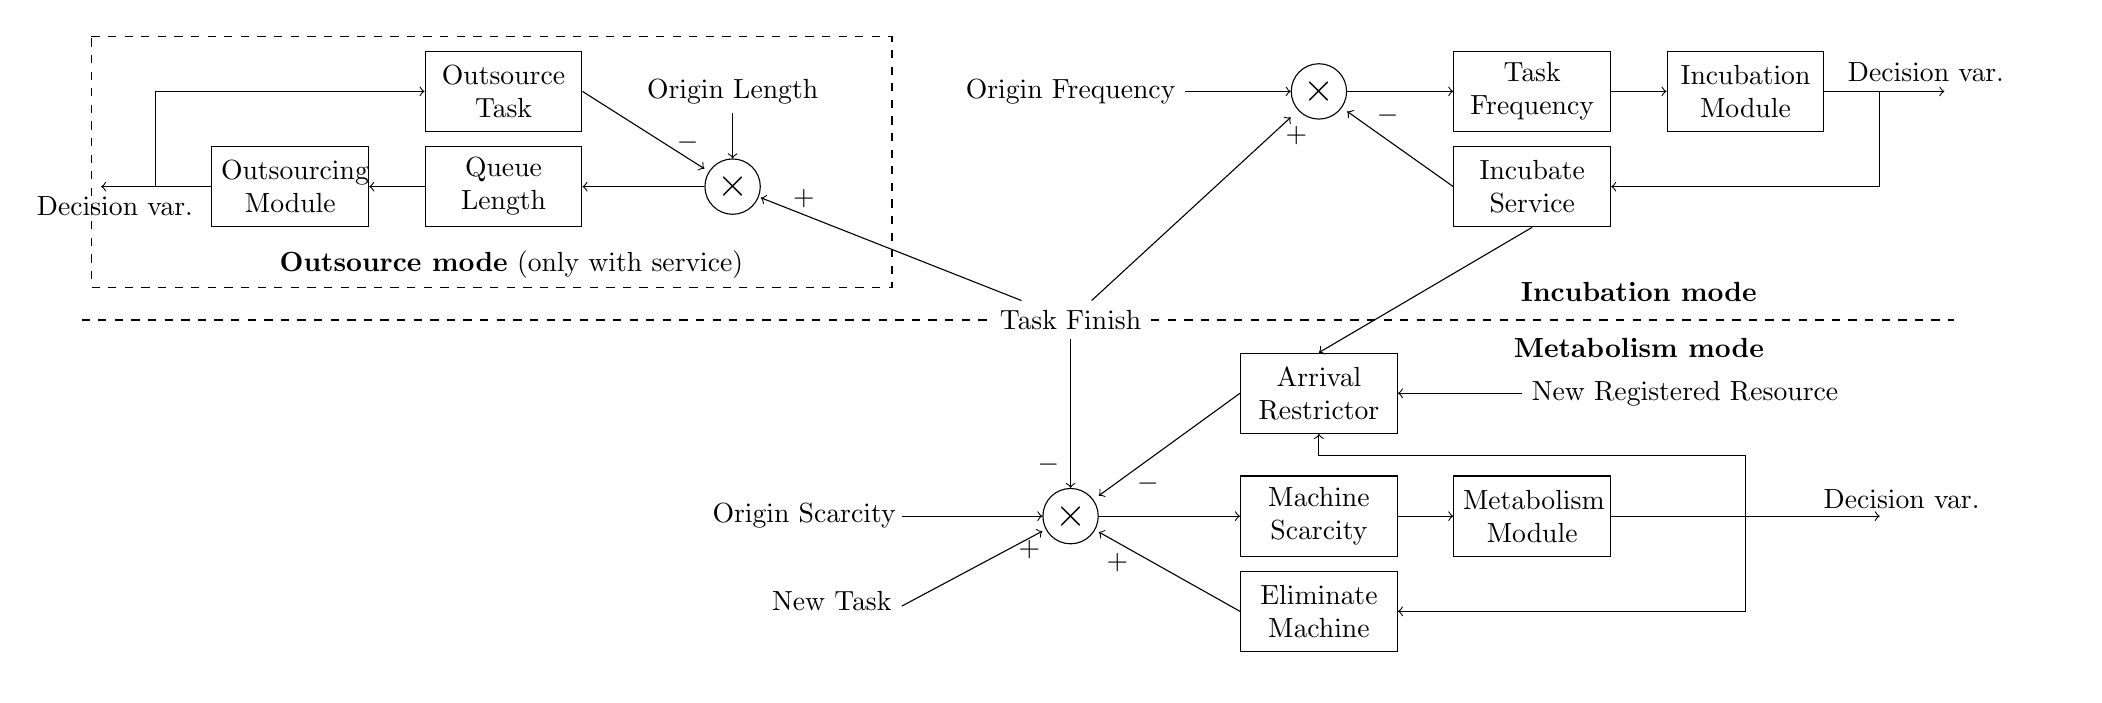
\begin{tikzpicture}[node distance=5mm and 5mm,
square/.style={
% The shape:
rectangle,
draw=black,
minimum size=2.9em,
text width=5em,
text centered
},
coord/.style={
coordinate,
% on chain,
% on grid,
% node distance=6mm and 25mm
},
circle/.style={
rectangle,minimum size=2em,rounded corners=1em,
draw=black
},
skip loop/.style={to path={-- ++(0,#1) -| (\tikztotarget)}}
]
\matrix[row sep=0.5em,column sep=2em] {
% First row:
\node (s1) [coord] {}; & & & & & \node (s2) [coord]{} ; & & & & & & \\
& & &   \node   (out) [square] {Outsource Task} ; &  \node (originl) {Origin Length} ; &  &\node (origin) {Origin Frequency} ; & \node (compare) [circle] {\Large$\times$}; &  \node (frequency) [square] {Task Frequency} ; & \node (incubate) [square] {Incubation Module} ; & \node (node) [coord] {} ; & \node (end) [coord] {}; \\
\node (end1)  {}; & \node (node1) [coord] {} ; & \node (outsource) [square] {Outsourcing Module} ; &\node (length) [square] {Queue Length} ; & \node (compare1) [circle] {\Large$\times$};  & & & & \node (sc) [square] {Incubate Service} ; & & & \\
\\
&& \node (o1){};& &\node (o2){}; \\
\node (s3) [coord]{}; &  & & & & \node (s4) [coord]{}; &  & & & & &\\
\node (tfs) {};& & \node (metam1) {};& &\node (metam2) {};& &  \node (tf) {Task Finish}; & &\node (incm1){}; & \node (incm2){};& &\node (tfe) {};\\
&&&&& & & \node (machinein) [square] {Arrival Restrictor}; & \node (add) {};  &  & &\\
&&&&&&&&&&&\\
&&&&&&&&&&&\\
& & && &\node (origin2) {};  & \node (compare2) [circle] {\Large$\times$}; &  \node (scarcity) [square] {Machine Scarcity}; & \node (metabolism) [square] {Metabolism Module}; &\node (node2) [coord] {}; &\node (end2) [coord] {};\\
&&&&&\node (task) {}; &  & \node (reduce) [square] {Eliminate Machine}; &  & & &\\
&&&&& &  &  & & & & &&  \\
};
\path (origin) edge[->] (compare) (tf) edge[->] (compare) (compare) edge[->] (frequency) (frequency) edge[->] (incubate) (incubate) edge[->] (end);
\path (sc.west) edge[->] (compare);
\draw [->] (node) |- (sc) ;
\path (tf) to node [near end,xshift=2em,yshift=1em] {$+$} (compare) (sc) to node [near end,xshift=0.5em] {$-$} (compare) (incubate) to node [yshift=0.7em,xshift = 1.5em] {Decision var.} (end);
\draw[dashed] (s1) -- (s2) -- (s4) -- (s3) -- (s1);
\draw[dashed,thick](tfs.west) -- (tf.west) (tf.east) -- (tfe.east);

\path (originl) edge[->] (compare1) (compare1) edge[->] (length) (length) edge[->] (outsource) (outsource) edge[->] (end1);
\path (out.east) edge[->] (compare1);
\draw [->] (node1) |- (out) ;
\path (out) to node [near end,xshift=0.5em,yshift=0.7em] {$-$} (compare1) (outsource) to node [near end,yshift=-0.7em,xshift = -0.5em] {Decision var.} (end1);

\draw[->] (tf) edge (compare1) (tf) edge (compare2);
\path (tf) to node [yshift=0.9em,xshift=-0.8em,near end] {$+$} (compare1) (tf) to node [xshift=-0.8em,yshift=-0.5em,near end] {$-$} (compare2);

\draw (sc.south) edge[->] (machinein.north);

\path (add) edge[->] (machinein) (machinein.west) edge[->] (compare2) (compare2) edge[->] (scarcity) (scarcity) edge[->] (metabolism);
\path (origin2) edge[->] (compare2);
% \path (tf) edge[->] (compare2);
\path (reduce.west)  edge[->] (compare2);
\draw [->] (metabolism) -- (end2) ;
\draw [->]  (task) -- (compare2);
\path (node2) edge[->,skip loop=2.2em] (machinein);
\draw [->] (node2) |- (reduce);
\path (machinein.west) to node [near end,yshift=-0.5em,xshift=0.5em] {$-$} (compare2);
% \path (tf) to node [near end,xshift=0.5em] {$-$} (compare2);
\path (task) to node [near end,xshift=0.8em] {$+$} (compare2);
\path (reduce) to node [near end,xshift=-0.6em,yshift=-0.8em] {$+$} (compare2);
\path (node2) to node [near end,xshift=2em,yshift=0.6em] {Decision var.} (end2);
\path (add) to node [near start, xshift=7em] {New Registered Resource}(machinein) (origin2) to node [near start,xshift=-4.8em]{Origin Scarcity}(compare2) (task) to node [near start,xshift=-3.8em,yshift=-0.5em]{New Task} (compare2);

\path (o1) to node {\textbf{Outsource mode} (only with service)} (o2);
\path (incm1) to node [yshift=1em]{\textbf{Incubation mode}} (incm2) (incm1) to node [yshift=-1em]{\textbf{Metabolism mode}} (incm2);
\end{tikzpicture}